\chapter{Program architecture}\label{sec:enterprise}

\section{Current situation in ReCodEx}

At the Faculty of Mathematics and Physics at the Charles University, the main platform for submitting programming assignments and exams is an online system called ReCodEx \cite{recodex}.
Teachers configure a set of test cases for each assignment, and the system automatically runs those tests to check the running time, memory usage, and correctness of the results of the submitted programs.

In homework assignments, students are able to search for solutions online and submit code written by AI tools.
But exams are taken in an offline environment, and the only source of plagiarism is then between students.

ReCodEx has a visual interface for teachers to see the results of the tests and the plagiarism reports.
The reports highlight similar code fragments between different files, grouped by the author of the submission.
The teachers can then inspect those fragments and decide whether the similarity is a case of plagiarism or not and what the appropriate next steps are.

A string-based plagiarism-detection tool Comparatrix \cite{comparatrix} is currently used in ReCodEx for C++ submissions.
It first removes comments and normalizes whitespace in the source code, and then collects $n$-grams of the resulting string.
These $n$-grams are searched for duplicates and identical code fragments are reported as similar.
If a file contains a large scope of code that is identical to fragments written by another author, it is reported as a case of plagiarism.
This approach does not do any syntactic or semantic analysis of the code, so the fragments do not correspond to syntactical structures.
The tool only detects identical code, so slightly modified code, for example with renamed identifiers, will not be detected at all.

At the end of each day, a batch of new files is sent to the plagiarism-detection tool, and the reports focusing on the new files (and their similarity to the new or old files) are generated and sent back to ReCodEx.
ReCodEx remembers all the reports and aggregates the results.

\section{Overall architecture}

The system consists of four main components:
\begin{itemize}
\item ReCodEx: The main platform for submitting programming assignments and exams, and it is responsible for receiving the source code files, running the tests, and showing the results to the teachers. It is the only component that interacts with the users.
\item atc (AST to comparatree, details in \autoref{sec:atc}): A tool for parsing the C/C++ source code files, extracting the relevant parts of the ASTs, and storing them in comparatree.
\item comparatree (details in \autoref{sec:comparatree}): A database for storing ASTs very efficiently together with metadata, with no need to store the original source code files.
\item ContrAST (details in \autoref{sec:contrast}): A tool for searching for similar code fragments in comparatree and generating reports that can be imported into ReCodEx.
\end{itemize}

The only component depending on the programming language of the assignments is atc.
If we want to support another language, we only need to implement a new atc for that language and add a short configuration into ContrAST, but the rest of the system can be reused without any modifications.

\begin{figure}[h]
    \centering
    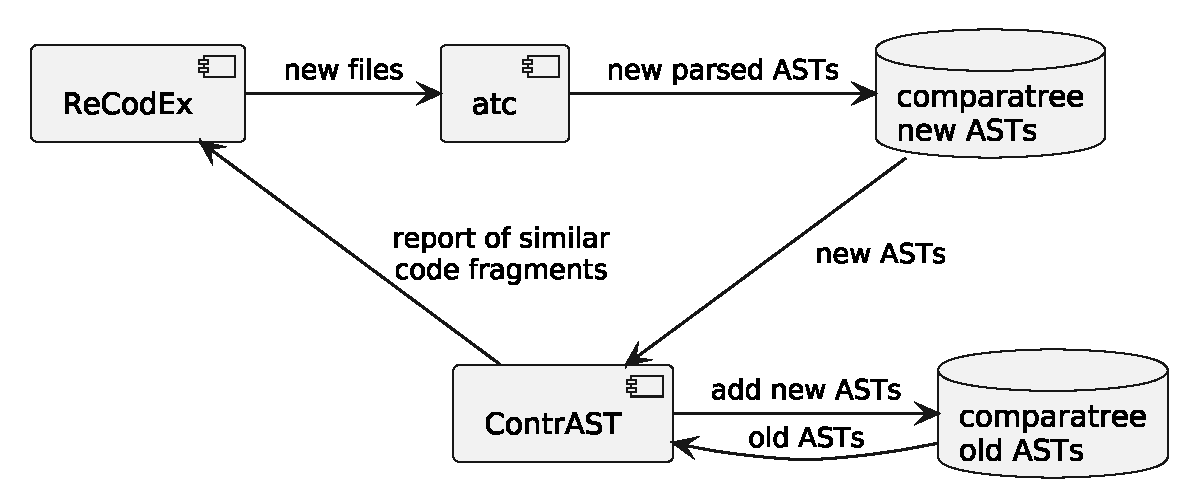
\includegraphics[width=\textwidth]{img/overall-architecture.eps}
    \caption{Data flow of the system.}
    \label{fig:overall-architecture}
\end{figure}

The data flow of the system can be seen in \autoref{fig:overall-architecture}.
As the new files are downloaded in batches, this process is repeated once per day.
One instance of comparatree is built per batch, and appended to one archive of all the previous batches.

There might exist multiple archive comparatree instances, one per assignment, for example, and the search for similar code fragments is then performed only on the one corresponding to the assignment.
It is up to the user to decide the organization of files into comparatree instances.

A set of Python scripts is used to automate the whole process, including downloading the files, running atc and ContrAST, and importing the results into ReCodEx.

ReCodEx has fixed interfaces for downloading data and importing reports, so the system needs to fit those requirements.
The main part is keeping the identifiers of the files (and also submissions and authors) consistent across the whole process.
As we do not want to store the original source code files and additional files outside of comparatree, all the metadata then must be stored in comparatree as well.
